% Provenance (never printed): see sources/outline_sources.md (Year 2: partial melting of the
% mantle; solidus and geotherm; decompression, hydration and heating; degree of melting;
% binary and ternary phase diagrams applied to rocks).
% Curves from figdata/bachelor-2/melting.py (Bowen 1915 diopside-anorthite, Bowen and
% Andersen 1914 forsterite-silica, Katz et al. 2003 melting of peridotite); exercise and
% problem values in the Book 4 scratch calculator calc/ch07.py.
\chapter{Melting the Mantle}\label{ch:b2:mantle-melting}

The mantle is solid. Seismic shear waves cross it from top to bottom, and the
\omterm{def:b2:mantle-melting:peridotites}{peridotite} brought up from it is a crystalline rock. Yet along the ocean ridges
alone it gives out some twenty cubic kilometres of new oceanic crust every year,
every cubic metre of it made from a melt. The paradox dissolves once one knows
that the mantle does not melt because it is heated: it melts because the
pressure on it falls, or because water is added to it. Beneath a ridge the
mantle rises, its pressure drops faster than its temperature, and it crosses its
melting curve; above a sinking slab, water released from the slab lowers that
curve under the mantle wedge. In both cases only a small fraction of the rock
melts, and that fraction, separated from its residue, becomes the basalt of the
ocean floor and of the volcanic arcs. This chapter first describes the mantle
rock and the phase diagrams that tell how such rocks melt, then follows the
mantle up beneath a ridge to the thickness of the crust it makes.
% ledger: white:crust (Book 3), data:pb2002 (Book 3), katz03:solidus

\begin{recall}
\textbf{From the chemistry books' Year 2 volume}: binary phase diagrams, the
solidus and the liquidus, the eutectic point, congruent melting, solid solutions
and the lever rule, by which the proportions of two coexisting phases are
inversely proportional to their distances from the bulk composition.
\textbf{From the physics books}: the specific heat, the latent heat, the entropy
and the second law, by which a reversible adiabatic process conserves entropy.
\textbf{From the Year 1 volume}: the main rock-forming minerals, olivine,
pyroxenes, garnet and spinel, their solid solutions and the Mg number; the
mantle adiabat, $\mathrm dT/\mathrm dz = \alpha gT/c_p$; the oceanic crust,
\qty[uncertainty-mode=separate]{7.1 \pm 0.8}{km} thick away from hotspots and
about \qty{20}{km} over the core of a plume; subducting slabs and the water they
carry. \textbf{From \cref{ch:b2:elements-in-the-earth}}: \omterm{def:b2:elements-in-the-earth:morb-oib}{mid-ocean ridge basalt}
(MORB), partition coefficients and \omterm{def:b2:elements-in-the-earth:partition}{incompatible elements}.
\end{recall}

\section{The mantle rock}\label{sec:b2:mantle-melting:rock}

Mantle rock reaches the surface as fragments carried up by \omterm{def:b2:magma-emplacement:magma}{magmas}, the
xenoliths, and as the base of slices of ocean lithosphere pushed onto the
continents, the ophiolites. Almost all of it is \omterm{def:b2:mantle-melting:peridotites}{peridotite}.
% ledger: geo:peridotite (Book 2), tulane:ocean-basins (Book 2)

\begin{definition}[Peridotite and its kinds]\label{def:b2:mantle-melting:peridotites}
A \emph{peridotite}\index{peridotite} is a coarse-grained ultramafic rock
containing more than \qty{40}{\percent} olivine, the rest being pyroxenes and a
little of an aluminous mineral (spinel or garnet). A
\emph{dunite}\index{dunite} contains more than \qty{90}{\percent} olivine. Below
that, a \emph{lherzolite}\index{lherzolite} contains both orthopyroxene and
clinopyroxene; a \emph{harzburgite}\index{harzburgite} contains orthopyroxene but
almost no clinopyroxene; a wehrlite contains clinopyroxene but almost no
orthopyroxene. Rocks with less than \qty{40}{\percent} olivine are pyroxenites.
\end{definition}
% ledger: bgs:ultramafic

The classification is read on a triangle whose corners are olivine,
orthopyroxene and clinopyroxene (the figure below): each point stands for a rock,
and its distances from the three sides give the proportions of the three
minerals. A model composition of the depleted upper mantle that melts beneath
the ridges has \qty{57}{\percent} olivine,
\qty{28}{\percent} orthopyroxene, \qty{13}{\percent} clinopyroxene and
\qty{2}{\percent} spinel: a \omterm{def:b2:mantle-melting:peridotites}{lherzolite}.
% ledger: liang21:dmm-mode

\begin{omfigure}
\centering
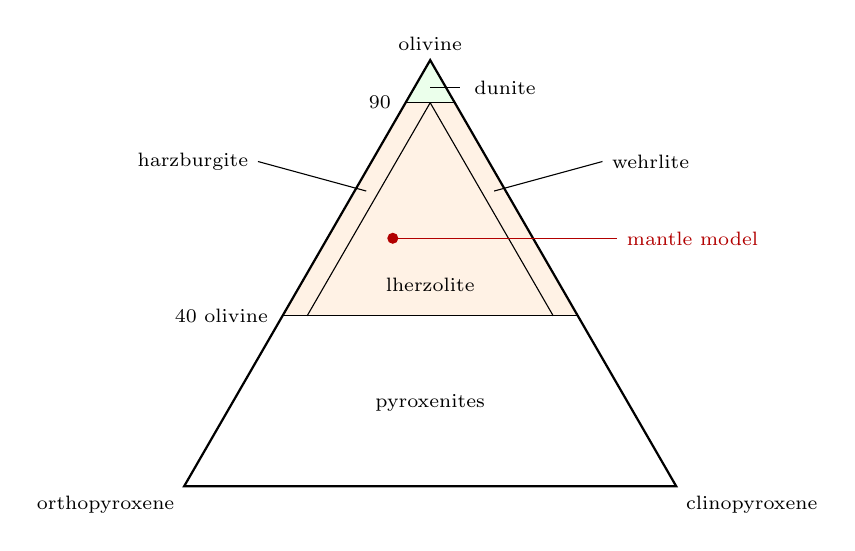
\begin{tikzpicture}[x=1.25cm, y=1.25cm, font=\scriptsize]
\coordinate (O) at (2.5,4.330); \coordinate (P) at (0,0); \coordinate (C) at (5,0);
\fill[green!8] (2.25,3.897) -- (2.75,3.897) -- (O) -- cycle;
\fill[orange!10] (1,1.732) -- (2.25,3.897) -- (2.75,3.897) -- (4,1.732) -- cycle;
\draw[thick] (O) -- (P) -- (C) -- cycle;
\draw (2.25,3.897) -- (2.75,3.897);
\draw (1,1.732) -- (4,1.732);
\draw (2.5,3.897) -- (1.25,1.732);
\draw (2.5,3.897) -- (3.75,1.732);
\node[anchor=south] at (O) {olivine};
\node[anchor=north east] at (P) {orthopyroxene};
\node[anchor=north west] at (C) {clinopyroxene};
\node[anchor=west] at (2.85,4.05) {dunite};
\draw (2.5,4.05) -- (2.8,4.05);
\node at (2.5,2.05) {lherzolite};
\draw (1.85,3.0) -- (0.75,3.3) node[anchor=east] {harzburgite};
\draw (3.15,3.0) -- (4.25,3.3) node[anchor=west] {wehrlite};
\node at (2.5,0.85) {pyroxenites};
\node[anchor=east] at (0.95,1.732) {\qty{40}{\percent} olivine};
\node[anchor=east] at (2.2,3.897) {\qty{90}{\percent}};
\fill[red!70!black] (2.12,2.52) circle (2pt);
\draw[red!70!black] (2.12,2.52) -- (4.4,2.52) node[anchor=west] {mantle model};
\end{tikzpicture}
\par\smallskip{\small Classification of the \omterm{def:b2:mantle-melting:peridotites}{peridotites} and pyroxenites by their
proportions of olivine, orthopyroxene and clinopyroxene (after the British
Geological Survey's scheme). The narrow strips along the two upper sides hold the
rocks with almost no clinopyroxene (\omterm{def:b2:mantle-melting:peridotites}{harzburgite}) or no orthopyroxene (wehrlite).
The red dot is the model upper mantle beneath the ridges (57, 28 and
\qty{13}{\percent}, renormalised without its \qty{2}{\percent} of spinel).}
\end{omfigure}
% ledger: bgs:ultramafic, liang21:dmm-mode

The three \omterm{def:b2:mantle-melting:peridotites}{peridotites} are not three independent rock types: they are stages of
one process. Clinopyroxene and the aluminous mineral are used up first when
\omterm{def:b2:mantle-melting:peridotites}{peridotite} melts (\cref{sec:b2:mantle-melting:decompression}), so a \omterm{def:b2:mantle-melting:peridotites}{lherzolite}
that has lost a melt becomes poorer in them; after enough melting it is a
\omterm{def:b2:mantle-melting:peridotites}{harzburgite}, and a rock that has lost almost all its pyroxene is a \omterm{def:b2:mantle-melting:peridotites}{dunite}.
% ledger: katz03:melting

\begin{definition}[Fertile and residual mantle]\label{def:b2:mantle-melting:fertility}
A \emph{fertile mantle}\index{fertile mantle} is a \omterm{def:b2:mantle-melting:peridotites}{peridotite}, typically a
\omterm{def:b2:mantle-melting:peridotites}{lherzolite}, that still contains the clinopyroxene and aluminous mineral from
which basalt is made. A \emph{residual mantle}\index{residual mantle} is the
\omterm{def:b2:mantle-melting:peridotites}{peridotite} left behind once a melt has been extracted from it: poorer in
clinopyroxene, aluminium, calcium and the \omterm{def:b2:elements-in-the-earth:partition}{incompatible elements}, richer in
olivine and with a higher Mg number.
\end{definition}

The isotopic \omterm{def:b2:isotope-geochemistry:reservoirs}{depleted mantle} of \cref{ch:b2:isotope-geochemistry} is a reservoir,
defined by its ratios; a \omterm{def:b2:mantle-melting:fertility}{residual mantle} is a rock, defined by what it has lost.
The two are linked, since the \omterm{def:b2:isotope-geochemistry:reservoirs}{depleted mantle} is depleted because melt was
extracted from it long ago, but one is read in a mass spectrometer and the other
under the microscope.

\section{Phase diagrams of rocks}\label{sec:b2:mantle-melting:diagrams}

A rock is a mixture of minerals, and it melts over a range of temperatures, not at
one point. The diagrams that describe this were first measured on mixtures of
pure synthetic minerals, by holding a small charge at a known temperature until it
reached equilibrium, quenching it, and looking under the microscope for glass,
which was liquid, and crystals.

\subsection*{A binary eutectic: diopside and anorthite}

A basalt consists essentially of a calcic plagioclase and a clinopyroxene, and
Bowen chose pure anorthite and diopside as its simplest model. Mixed and heated,
they form an ordinary eutectic
system (the figure below): diopside melts at \qty{1391.5}{\celsius} and anorthite
at \qty{1550}{\celsius}, but a mixture of \qty{58}{\percent} diopside and
\qty{42}{\percent} anorthite by mass melts completely at \qty{1270}{\celsius}.
% ledger: bowen15:di-an

\begin{omfigure}
\centering
\begin{tikzpicture}
\begin{axis}[omrecord, width=0.78\linewidth, height=6cm,
  xmin=0, xmax=100, ymin=1200, ymax=1600,
  xlabel={anorthite (\unit{\percent} by mass)}, ylabel={temperature (\unit{\celsius})},
  y tick label style={/pgf/number format/1000 sep={}},
  tick label style={font=\scriptsize}, label style={font=\small}]
\addplot[very thick, black] table[x=x_an, y=T] {figdata/out/bachelor-2-melting-di-an-liq.dat};
\addplot[only marks, mark=*, mark size=1.6pt, blue!70!black] table[x=x_an, y=T] {figdata/out/bachelor-2-melting-di-an-data.dat};
\draw[thick] (axis cs:0,1270) -- (axis cs:100,1270);
\draw[densely dotted, red!70!black, thick] (axis cs:20,1590) -- (axis cs:20,1270);
\draw[->, red!70!black, thick] (axis cs:20,1350) -- (axis cs:41,1272);
\fill[red!70!black] (axis cs:20,1350) circle (1.6pt);
\node[font=\scriptsize] at (axis cs:55,1500) {liquid};
\node[font=\scriptsize, align=center] at (axis cs:10,1300) {diopside\\+ liquid};
\node[font=\scriptsize, align=center] at (axis cs:72,1360) {anorthite + liquid};
\node[font=\scriptsize] at (axis cs:68,1235) {diopside + anorthite};
\node[font=\scriptsize, anchor=north east] at (axis cs:41,1267) {E, \qty{1270}{\celsius}};
\node[font=\scriptsize, anchor=west, red!70!black] at (axis cs:21,1360) {first diopside};
\end{axis}
\end{tikzpicture}
\par\smallskip{\small The system diopside--anorthite at atmospheric pressure, from
the quenching experiments of Bowen (1915): liquidus temperatures (dots, midpoints of
the quenching brackets) and the eutectic E. In red, the cooling of a liquid of
\qty{20}{\percent} anorthite: diopside crystallises from \qty{1350}{\celsius}, the
liquid moves down the liquidus to E, and the rest crystallises there as a mixture of
both minerals.}
\end{omfigure}
% ledger: bowen15:di-an

Read from above, the diagram tells the order of crystallisation. A liquid of
\qty{20}{\percent} anorthite begins to crystallise diopside at
\qty{1350}{\celsius}; the liquid, losing diopside, grows richer in anorthite and
moves down the liquidus until it reaches the eutectic, where anorthite joins
diopside and the temperature stays at \qty{1270}{\celsius} until all the liquid is
gone. Read from below, it tells how the rock melts: whatever the proportions of
the two minerals, the first liquid appears at \qty{1270}{\celsius} and has the
eutectic composition. That is the first lesson for the mantle. The first melt of a
rock does not have the rock's composition: it has the composition fixed by the
minerals it melts from, and it appears at a temperature well below the melting
points of all of them.

\subsection*{Incongruent melting: forsterite and silica}

Some minerals do not melt into a liquid of their own composition.

\begin{definition}[Incongruent melting, peritectic point]\label{def:b2:mantle-melting:peritectic}
A mineral shows \emph{incongruent melting}\index{incongruent melting} when, on
heating, it breaks down into another solid and a liquid of a different
composition, instead of melting into a liquid of its own composition. On a binary
phase diagram, the point where that liquid coexists with both solids is a
\emph{peritectic point}\index{peritectic point}: unlike a eutectic, it does not lie
between the compositions of the two solids.
\end{definition}

Enstatite, the magnesian orthopyroxene \ce{MgSiO3}, melts incongruently. At
atmospheric pressure it breaks down at \qty{1557}{\celsius} into forsterite,
\ce{Mg2SiO4}, and a liquid slightly richer in silica than itself; only at
\qty{1577}{\celsius} has all the forsterite dissolved (the figure below). Bowen
and Andersen found in 1914 that the breakdown gives \qty{5.5}{\percent} of
forsterite and \qty{94.5}{\percent} of liquid, as the lever rule predicts from
the three compositions (\cref{exo:b2:mantle-melting:6}). Further toward silica, enstatite and
cristobalite melt together at a eutectic, \qty{1543}{\celsius}.
% ledger: bowen14:mgo-sio2

\begin{omfigure}
\centering
\begin{tikzpicture}
\begin{axis}[omrecord, width=0.78\linewidth, height=6cm,
  xmin=40, xmax=66, ymin=1450, ymax=1950,
  xlabel={\ce{SiO2} (\unit{\percent} by mass)}, ylabel={temperature (\unit{\celsius})},
  y tick label style={/pgf/number format/1000 sep={}},
  tick label style={font=\scriptsize}, label style={font=\small}]
\addplot[very thick, black] table[x=x_sio2, y=T] {figdata/out/bachelor-2-melting-fo-sio2-liq.dat};
\addplot[very thick, black, dashed] table[x=x_sio2, y=T] {figdata/out/bachelor-2-melting-fo-sio2-fo.dat};
\draw[thick] (axis cs:42.71,1450) -- (axis cs:42.71,1890);
\draw[thick] (axis cs:42.71,1557) -- (axis cs:60.86,1557);
\draw[thick] (axis cs:59.85,1450) -- (axis cs:59.85,1557);
\draw[thick] (axis cs:59.85,1543) -- (axis cs:66,1543);
\fill (axis cs:60.86,1557) circle (1.6pt);
\fill (axis cs:64.87,1543) circle (1.6pt);
\fill (axis cs:42.71,1890) circle (1.6pt);
\node[font=\scriptsize, anchor=south west] at (axis cs:42.9,1890) {forsterite melts, \qty{1890}{\celsius}};
\node[font=\scriptsize] at (axis cs:56,1800) {liquid};
\node[font=\scriptsize] at (axis cs:48,1680) {forsterite + liquid};
\node[font=\scriptsize] at (axis cs:51,1500) {forsterite + enstatite};
\node[font=\scriptsize, align=center] at (axis cs:63,1495) {enstatite +\\cristobalite};
\node[font=\scriptsize, anchor=south] at (axis cs:61.3,1560) {P};
\node[font=\scriptsize, anchor=south] at (axis cs:64.87,1546) {E};
\node[font=\scriptsize, anchor=north, rotate=90] at (axis cs:42.71,1650) {\ce{Mg2SiO4}};
\node[font=\scriptsize, anchor=south, rotate=90] at (axis cs:59.85,1510) {\ce{MgSiO3}};
\end{axis}
\end{tikzpicture}
\par\smallskip{\small Part of the system \ce{MgO}--\ce{SiO2} at atmospheric
pressure, from Bowen and Andersen (1914). Enstatite (\ce{MgSiO3}) melts
incongruently at the peritectic P, \qty{1557}{\celsius}, into forsterite and a
liquid of \qty{60.9}{\percent} \ce{SiO2}; E is the enstatite--cristobalite
eutectic, \qty{1543}{\celsius}. The forsterite liquidus is measured only near
enstatite: the dashed part is drawn straight to the melting point of forsterite.}
\end{omfigure}
% ledger: bowen14:mgo-sio2

The peritectic is the second lesson for the mantle. When a \omterm{def:b2:mantle-melting:peridotites}{peridotite} melts, its
orthopyroxene does not simply dissolve: it gives olivine to the residue and silica
to the melt. The melt is therefore richer in silica than the pyroxenes, and the
residue richer in olivine than the rock: the path from \omterm{def:b2:mantle-melting:peridotites}{lherzolite} to \omterm{def:b2:mantle-melting:peridotites}{harzburgite}
and \omterm{def:b2:mantle-melting:peridotites}{dunite}.

\subsection*{Three components: the ternary diagram}

Real rocks have more than two minerals. With three, the composition needs a
triangle, and temperature becomes a third dimension.

\begin{definition}[Ternary phase diagram, cotectic line, ternary eutectic]\label{def:b2:mantle-melting:ternary}
A \emph{ternary phase diagram}\index{ternary phase diagram} represents the
equilibria of a system of three components at a given pressure: each point of a
triangle stands for a composition, the corners for the pure components, and the
liquidus surface is drawn as contours of temperature or as the fields of the
minerals that crystallise first. A \emph{cotectic line}\index{cotectic line} is
the line along which the liquid is saturated in two minerals at once and
crystallises both as it cools. The cotectic lines descend from the binary
eutectics on the sides of the triangle and meet at the \emph{ternary
eutectic}\index{ternary eutectic}, the lowest temperature at which liquid exists,
where the three minerals crystallise together.
\end{definition}

\begin{method}[Reading a crystallisation path on a ternary diagram]\label{met:b2:mantle-melting:ternary}
Locate the bulk composition $X$ in the triangle and the field in which it lies:
that field's mineral crystallises first. While that mineral alone crystallises,
the liquid moves in a straight line directly away from the mineral's corner,
through $X$, because removing a pure component changes only its proportion; by the
lever rule the mass fraction of crystals is the distance from $X$ to the liquid
divided by the distance from the corner to the liquid. When the liquid reaches a
\omterm{def:b2:mantle-melting:ternary}{cotectic line}, the second mineral joins and the liquid follows the cotectic
downhill to the \omterm{def:b2:mantle-melting:ternary}{ternary eutectic}, where the last liquid crystallises. A component
that enters none of the crystals stays in the liquid, so its concentration gives
the fraction of liquid left: $f_{\text{liquid}} = c_X/c_{\text{liquid}}$.
\end{method}

\begin{omfigure}
\centering
\begin{tikzpicture}[x=1cm, y=1cm, font=\scriptsize]
\coordinate (A) at (3,5.196); \coordinate (B) at (0,0); \coordinate (C) at (6,0);
\coordinate (eAB) at (1.2,2.078); \coordinate (eAC) at (4.65,2.338);
\coordinate (eBC) at (3.9,0); \coordinate (E) at (3.45,1.299);
\coordinate (X) at (3.0,3.118); \coordinate (L) at (3.0,1.455);
\fill[green!8] (A) -- (eAB) -- (E) -- (eAC) -- cycle;
\fill[orange!10] (B) -- (eAB) -- (E) -- (eBC) -- cycle;
\fill[blue!7] (C) -- (eAC) -- (E) -- (eBC) -- cycle;
\draw[thick] (A) -- (B) -- (C) -- cycle;
\draw[very thick, -{Stealth[length=4pt]}] (eAB) -- ($(eAB)!0.55!(E)$);
\draw[very thick] ($(eAB)!0.5!(E)$) -- (E);
\draw[very thick, -{Stealth[length=4pt]}] (eAC) -- ($(eAC)!0.55!(E)$);
\draw[very thick] ($(eAC)!0.5!(E)$) -- (E);
\draw[very thick, -{Stealth[length=4pt]}] (eBC) -- ($(eBC)!0.55!(E)$);
\draw[very thick] ($(eBC)!0.5!(E)$) -- (E);
\draw[red!70!black, thick, dashed] (A) -- (X);
\draw[red!70!black, very thick, -{Stealth[length=4pt]}] (X) -- (L);
\draw[red!70!black, very thick, -{Stealth[length=4pt]}] (L) -- ($(L)!0.85!(E)$);
\fill[red!70!black] (X) circle (2pt); \fill[red!70!black] (L) circle (1.6pt);
\fill (E) circle (2pt);
\node[anchor=south] at (A) {A}; \node[anchor=north east] at (B) {B};
\node[anchor=north west] at (C) {C};
\node[anchor=west, red!70!black] at (3.1,3.2) {$X$};
\node[anchor=north east, red!70!black] at (2.95,1.42) {$L_1$};
\node[anchor=north west] at (3.5,1.25) {E};
\node[anchor=east] at (eAB) {$e_{AB}$}; \node[anchor=west] at (eAC) {$e_{AC}$};
\node[anchor=north] at (eBC) {$e_{BC}$};
\node at (2.35,2.75) {A field}; \node at (1.55,0.7) {B field}; \node at (4.9,0.7) {C field};
\end{tikzpicture}
\par\smallskip{\small A \omterm{def:b2:mantle-melting:ternary}{ternary eutectic} system (schematic). Each field holds
the liquids from which its mineral crystallises first; the \omterm{def:b2:mantle-melting:ternary}{cotectic lines} (arrows
towards falling temperature) run from the binary eutectics $e$ to the \omterm{def:b2:mantle-melting:ternary}{ternary
eutectic} E. A liquid $X$ in the A field crystallises A, and moves away from the A
corner until it meets the A--B cotectic at $L_1$; A and B then crystallise
together down to E, where C joins them (\cref{exo:b2:mantle-melting:11}).}
\end{omfigure}

Systems of three rock-forming minerals are read in the same way. The rules that fix how many phases can coexist,
and the free-energy surfaces from which such diagrams are computed, belong to the
Year 3 volume of this series.

\section{Solidus, adiabat and three ways to melt}\label{sec:b2:mantle-melting:solidus}

Mantle \omterm{def:b2:mantle-melting:peridotites}{peridotite} has a solidus, the temperature at which its first melt appears,
and a liquidus far above it. Both rise with pressure. Experiments on natural
\omterm{def:b2:mantle-melting:peridotites}{peridotites}, compiled and fitted by Katz, Spiegelman and Langmuir in 2003, give
for the dry solidus
\[
  T_{\mathrm{s}}(P) = 1085.7 + 132.9\,P - 5.1\,P^2
\]
(in degrees Celsius, $P$ in gigapascals): \qty{1086}{\celsius} at the surface,
\qty{1331}{\celsius} at \qty{2}{GPa}. At the same depths the mantle is hotter or
colder than this depending on where it is, and to compare mantles one removes the
effect of depth.
% ledger: katz03:solidus

\begin{definition}[Mantle potential temperature]\label{def:b2:mantle-melting:tp}
The \emph{mantle potential temperature}\index{mantle potential temperature} $T_p$
is the temperature that a parcel of convecting mantle would have if it were
brought up to the surface along the mantle adiabat, without exchanging heat and
without melting.
\end{definition}

Along the adiabat $\mathrm dT/\mathrm dP = \alpha T/(\rho c_p)$, the form in
pressure of the gradient $\alpha gT/c_p$ recalled above, since $\mathrm dP = \rho
g\,\mathrm dz$. With $\alpha = \qty{4e-5}{K^{-1}}$, $\rho = \qty{3300}{kg/m^3}$
and $c_p = \qty{1000}{J/(kg.K)}$, it is about \qty{20}{K} per gigapascal, a
gigapascal being \qty{30.9}{km} of mantle (\cref{exo:b2:mantle-melting:3}). The Year 1 volume gave
the mantle a potential temperature of about \qty{1350}{\celsius} from mineral
physics; petrological estimates for the mantle beneath ridges range from 1280 to
\qty{1400}{\celsius}.
% ledger: katz03:thermo, katsura:adiabat (Book 3), herzberg:tp (Book 3)

\begin{proposition}[Onset of decompression melting]\label{prop:b2:mantle-melting:onset}
Mantle of potential temperature $T_p$ rising along the adiabat $T = T_p + GP$ ($G$
constant) begins to melt at the pressure $P_0$ where the adiabat meets the
solidus $T_{\mathrm s}(P) = a_1 + a_2P + a_3P^2$, the smaller root of
\[
  -a_3P^2 + (G - a_2)P + (T_p - a_1) = 0 .
\]
A mantle hotter by $\Delta T_p$ begins to melt deeper, by $\Delta P_0 \approx
\Delta T_p/(T_{\mathrm s}'(P_0) - G)$.
\end{proposition}

\begin{proof}
At depth the adiabat is colder than the solidus, because the solidus rises more
steeply ($T_{\mathrm
s}' \approx \qty{110}{K/GPa}$ against $G \approx 20$). The two curves cross where
$T_p + GP = a_1 + a_2P + a_3P^2$, which rearranges into the quadratic. Differentiating
$T_p + GP_0 = T_{\mathrm s}(P_0)$ gives $\mathrm dT_p = (T_{\mathrm s}'(P_0) -
G)\,\mathrm dP_0$.
\end{proof}

For $T_p = \qty{1350}{\celsius}$ the onset is at \qty{2.66}{GPa}, about
\qty{82}{km} down, at \qty{1403}{\celsius}; every \qty{10}{\celsius} of potential
temperature moves it by about \qty{0.12}{GPa}, or \qty{3.6}{km}. The figure below
shows the solidus and the adiabats.

\begin{omfigure}
\centering
\begin{tikzpicture}
\begin{axis}[omrecord, width=0.8\linewidth, height=7cm,
  xmin=850, xmax=2000, ymin=0, ymax=6, y dir=reverse,
  xlabel={temperature (\unit{\celsius})}, ylabel={pressure (\unit{GPa})},
  x tick label style={/pgf/number format/1000 sep={}},
  axis y line*=left,
  legend style={font=\scriptsize, at={(0.5,-0.2)}, anchor=north, legend columns=3},
  tick label style={font=\scriptsize}, label style={font=\small}]
\addplot[very thick, black] table[x=Ts, y=P_GPa] {figdata/out/bachelor-2-melting-pt.dat};
\addlegendentry{dry solidus}
\addplot[thick, black, densely dotted] table[x=Tl, y=P_GPa] {figdata/out/bachelor-2-melting-pt.dat};
\addlegendentry{lherzolite liquidus}
\addplot[thick, black, dashed] table[x=Tq, y=P_GPa] {figdata/out/bachelor-2-melting-pt.dat};
\addlegendentry{liquidus}
\addplot[thick, blue!70!black, dashdotted] table[x=wetsat, y=P_GPa] {figdata/out/bachelor-2-melting-pt.dat};
\addlegendentry{water-saturated solidus}
\addplot[thick, red!70!black] table[x=ad1350, y=P_GPa] {figdata/out/bachelor-2-melting-pt.dat};
\addlegendentry{adiabats, $T_p$ = 1300, 1350, \qty{1450}{\celsius}}
\addplot[thin, red!70!black] table[x=ad1300, y=P_GPa] {figdata/out/bachelor-2-melting-pt.dat};
\addplot[thin, red!70!black] table[x=ad1450, y=P_GPa] {figdata/out/bachelor-2-melting-pt.dat};
\addplot[only marks, mark=*, mark size=2pt, red!70!black] table[x=T0, y=P0] {figdata/out/bachelor-2-melting-onset.dat};
\end{axis}
\begin{axis}[width=0.8\linewidth, height=7cm, xmin=850, xmax=2000,
  ymin=0, ymax=185.34, y dir=reverse, axis y line*=right, axis x line=none,
  ylabel={depth (\unit{km})}, tick label style={font=\scriptsize}, label style={font=\small}]
\end{axis}
\end{tikzpicture}
\par\smallskip{\small Melting curves of dry \omterm{def:b2:mantle-melting:peridotites}{peridotite} and the water-saturated
solidus from the parameterisation of Katz and others (2003), with solid adiabats
for three potential temperatures; the dots mark the onset of melting,
\qty{2.08}{GPa} for \qty{1300}{\celsius}, \qty{2.66}{GPa} for
\qty{1350}{\celsius} and \qty{4.00}{GPa} for \qty{1450}{\celsius}. Between the
solidus and the \omterm{def:b2:mantle-melting:peridotites}{lherzolite} liquidus the rock melts while it keeps its
clinopyroxene. Depth scale for a mantle of \qty{3300}{kg/m^3}.}
\end{omfigure}
% ledger: katz03:solidus, katz03:water, katz03:thermo

The diagram shows the three ways to bring a rock above its solidus.

\begin{definition}[Partial, decompression and flux melting]\label{def:b2:mantle-melting:melting}
\emph{Partial melting}\index{partial melting} is the melting of a fraction of a
rock, between its solidus and its liquidus. \emph{Decompression
melting}\index{decompression melting} is the partial melting of rock that rises,
and so loses pressure, faster than it cools, until it crosses its solidus.
\emph{Flux melting}\index{flux melting}\index{hydrous melting|see{flux melting}},
or hydrous melting, is the partial melting caused by the addition of a volatile,
chiefly water, which lowers the solidus below the rock's temperature. The third
way, heating a rock above its solidus at constant pressure, needs an outside
source of heat, such as a hot \omterm{def:b2:magma-emplacement:magma}{magma}.
\end{definition}

Heating is the least efficient in the mantle, which conducts heat slowly; in the
crust, the heat of basaltic \omterm{def:b2:magma-emplacement:magma}{magma} can melt the rocks around it
(\cref{ch:b2:crustal-melting}). Decompression feeds the ridges and the hotspots;
\omterm{def:b2:mantle-melting:melting}{flux melting} feeds the volcanic arcs.

\section{Decompression melting beneath a ridge}\label{sec:b2:mantle-melting:decompression}

Once the rising mantle crosses its solidus, it keeps rising, and the question
becomes how much melt it makes.

\begin{definition}[Melt fraction]\label{def:b2:mantle-melting:fraction}
The \emph{melt fraction}\index{melt fraction} $F$ of a partially molten rock is
the mass of melt it has produced divided by its initial mass. Between the solidus
($F = 0$) and the liquidus ($F = 1$), the temperature on the melting surface is a
function $T(P, F)$.
\end{definition}

Melting takes heat: the latent heat, $T\Delta S$ per kilogram of melt, where
$\Delta S$ is the entropy of melting. A rising parcel exchanges no heat with its
surroundings, so the latent heat comes from its own temperature, and it rises
along a path of constant entropy that lies between the solidus and the liquidus.

\begin{proposition}[Isentropic melt productivity]\label{prop:b2:mantle-melting:productivity}
For mantle rising without exchanging heat, with specific heat $c_p$, thermal
expansivity $\alpha$, density $\rho$ and entropy of melting $\Delta S$, the
\emph{melt productivity}\index{melt productivity}, the melt made per unit fall of
pressure, is
\[
  -\frac{\mathrm dF}{\mathrm dP} =
  \frac{\dfrac{c_p}{T}\Big(\dfrac{\partial T}{\partial P}\Big)_F - \dfrac{\alpha}{\rho}}
       {\Delta S + \dfrac{c_p}{T}\Big(\dfrac{\partial T}{\partial F}\Big)_P}\,,
\]
with $T$ in kelvins.
\end{proposition}

\begin{proof}
The specific entropy of the partially molten rock changes by $\mathrm ds = c_p\,
\mathrm dT/T - (\alpha/\rho)\,\mathrm dP + \Delta S\,\mathrm dF$: the first two
terms are those of a solid (the second is a Maxwell relation, recalled from the
physics books), the third is the entropy gained by the mass $\mathrm dF$ that
melts. A reversible adiabatic ascent keeps $\mathrm ds = 0$. On the melting
surface $\mathrm dT = (\partial T/\partial P)_F\,\mathrm dP + (\partial
T/\partial F)_P\,\mathrm dF$. Substituting,
\[
  \Big[\frac{c_p}{T}\Big(\frac{\partial T}{\partial P}\Big)_F - \frac{\alpha}{\rho}\Big]\mathrm dP
  + \Big[\Delta S + \frac{c_p}{T}\Big(\frac{\partial T}{\partial F}\Big)_P\Big]\mathrm dF = 0,
\]
which is the result.
\end{proof}

The numerator is the excess of the melting curves' slope over the adiabat's, the
drive; the denominator holds the latent heat and the heat needed to raise the
temperature of the melting rock along the melting interval, the brakes. With the
parameters of Katz and others, $\Delta S = \qty{300}{J/(kg.K)}$, and a \omterm{def:b2:mantle-melting:fraction}{melt
fraction} that rises linearly between the solidus and the \omterm{def:b2:mantle-melting:peridotites}{lherzolite} liquidus, the
productivity at \qty{2}{GPa} is about \qty{11}{\percent} per gigapascal
(\cref{exo:b2:mantle-melting:8}): each kilometre of ascent melts about a third of a per cent of the
rock. Their fitted melting function, which makes the first per cent of melt come
slowly, gives a little less on average, about \qty{9}{\percent} per gigapascal
from the onset to the surface for $T_p = \qty{1350}{\celsius}$. The productivity
drops when clinopyroxene is used up, after \omterm{def:b2:mantle-melting:fraction}{melt fractions} of
$M_{\mathrm{cpx}}/(0.50 + 0.08P)$ in their model, some 25 to \qty{30}{\percent} for
a mantle with 13 to \qty{15}{\percent} clinopyroxene: a \omterm{def:b2:mantle-melting:peridotites}{harzburgite} residue melts
reluctantly.
% ledger: katz03:melting, katz03:thermo

\begin{omfigure}
\centering
\begin{tikzpicture}
\begin{axis}[omrecord, width=0.62\linewidth, height=6.4cm,
  xmin=0, xmax=0.36, ymin=0, ymax=130, y dir=reverse,
  xlabel={melt fraction $F$}, ylabel={depth (\unit{km})},
  xtick={0,0.1,0.2,0.3},
  legend style={font=\scriptsize, at={(0.98,0.02)}, anchor=south east},
  tick label style={font=\scriptsize}, label style={font=\small}]
\addplot[thick, blue!70!black] table[x=F1300, y=z_km] {figdata/out/bachelor-2-melting-column.dat};
\addlegendentry{$T_p = \qty{1300}{\celsius}$}
\addplot[very thick, black] table[x=F1350, y=z_km] {figdata/out/bachelor-2-melting-column.dat};
\addlegendentry{$T_p = \qty{1350}{\celsius}$}
\addplot[thick, red!70!black, dashed] table[x=F1450, y=z_km] {figdata/out/bachelor-2-melting-column.dat};
\addlegendentry{$T_p = \qty{1450}{\celsius}$}
\end{axis}
\end{tikzpicture}
\par\smallskip{\small \omterm{def:b2:mantle-melting:fraction}{Melt fraction} of a column of dry \omterm{def:b2:mantle-melting:peridotites}{peridotite} rising without
exchanging heat, from the onset of melting to the surface, computed by conserving
entropy with the melting function of Katz and others (2003), for a rock with
\qty{15}{\percent} clinopyroxene. At \qty{1450}{\celsius} the clinopyroxene is used
up near \qty{25}{km} and the curve steepens.}
\end{omfigure}
% ledger: katz03:melting, katz03:thermo

The melt does not stay where it forms. At about \qty{2900}{kg/m^3} it is
lighter than the solid \omterm{def:b2:mantle-melting:peridotites}{peridotite}, \qty{3300}{kg/m^3}, so it separates from its
residue and rises through it; beneath a ridge it is gathered towards the axis.
The crust is built from the melts of a whole region of the mantle.
% ledger: katz03:thermo

\begin{proposition}[Crust of a triangular melting region]\label{prop:b2:mantle-melting:triangle}
Beneath a ridge spreading at the half-rate $U$, let the mantle rise vertically at
the speed $U$ through a triangular melting region of height $H$, apex at the top
beneath the axis and sides at \ang{45}, and leave it horizontally at the speed $U$
across its sides; let the \omterm{def:b2:mantle-melting:fraction}{melt fraction} grow linearly from $0$ at the base to
$F_{\max}$ at the apex, all the melt be extracted to the crust, and mantle and
crust have the same density. Then the crust is
\[
  h_c = \int_0^H F(z)\,\mathrm dz = \tfrac12 F_{\max}H
\]
thick, and the aggregated melt has the mean \omterm{def:b2:mantle-melting:fraction}{melt fraction} $F_{\max}/2$.
\end{proposition}

\begin{proof}
Measure $x$ from the axis and the height $y$ above the base. Mantle enters the base
at $|x| \le H$ and rises until it meets a side, at $y = H - |x|$, having melted to
$F = F_{\max}(H - |x|)/H$. Per unit length of ridge and unit time, the melt made is
$\int_{-H}^{H} U F\,\mathrm dx = 2UF_{\max}\int_0^H (1 - x/H)\,\mathrm dx =
UF_{\max}H$. The crust leaves on both sides at the speed $U$: $2Uh_c = UF_{\max}H$.
The mantle processed is $2UH$, so the mean \omterm{def:b2:mantle-melting:fraction}{melt fraction} is $UF_{\max}H/(2UH) =
F_{\max}/2$. Finally $\int_0^H F_{\max}\,y/H\,\mathrm dy = F_{\max}H/2$.
\end{proof}

The result does not depend on the spreading rate, as observed (the Year 1
volume). For $T_p = \qty{1350}{\celsius}$ the column of the figure above, with its
slow start, gives $\int F\,\mathrm dz = \qty{9.0}{km}$ of crust, a little more
than the \qty{7.1}{km} measured; a mantle \qty{50}{\celsius} colder gives
\qty{5.5}{km}, and one \qty{100}{\celsius} hotter \qty{19}{km}, close to the
\qty{20}{km} over the core of a plume (the figure below). Crustal thickness is a
thermometer, and a sensitive one: since $h_c \propto P_0^2$ when productivity is
constant, ten degrees change it by about a tenth (weekend problem).
% ledger: white:crust (Book 3)

\begin{omfigure}
\centering
\begin{tikzpicture}[x=1cm, y=1cm, font=\scriptsize]
\fill[blue!8] (-5.5,0.6) rectangle (5.5,0);
\fill[brown!35] (-5.5,0) -- (5.5,0) -- (5.5,-0.35) -- (-5.5,-0.35) -- cycle;
\fill[orange!25] (0,-0.45) -- (-3.6,-4.05) -- (3.6,-4.05) -- cycle;
\draw[densely dashed, thick] (-5.5,-4.05) -- (5.5,-4.05);
\node[anchor=north east] at (5.5,-4.55) {solidus crossed: melting begins, depth $z_0$};
\foreach \s in {1,-1} {
  \draw[->, thick] (\s*0.4,0.35) -- (\s*1.6,0.35);
  \draw[gray, -{Stealth[length=3pt]}] (\s*1.8,-4.5) -- (\s*1.8,-2.45) .. controls (\s*1.8,-2.1) and (\s*2.1,-1.95) .. (\s*2.8,-1.95) -- (\s*5.3,-1.95);
  \draw[gray, -{Stealth[length=3pt]}] (\s*3.1,-4.5) -- (\s*3.1,-3.75) .. controls (\s*3.1,-3.4) and (\s*3.4,-3.25) .. (\s*4.1,-3.25) -- (\s*5.3,-3.25);
}
\draw[red!70!black, -{Stealth[length=3pt]}, thick] (-1.2,-3.0) -- (-0.3,-1.0);
\draw[red!70!black, -{Stealth[length=3pt]}, thick] (1.2,-3.0) -- (0.3,-1.0);
\draw[red!70!black, -{Stealth[length=3pt]}, thick] (0,-2.3) -- (0,-0.9);
\node[anchor=south] at (0,0.6) {ridge axis};
\node[anchor=west] at (1.7,0.35) {plate, speed $U$};
\node[anchor=west] at (-5.4,-0.2) {crust, $h_c$};
\node[align=center, inner sep=1pt] at (0,-3.3) {melting region};
\node[anchor=west, align=left] at (3.2,-2.55) {flow lines of\\the mantle};
\node[anchor=east, align=right, red!70!black] at (-2.0,-2.6) {melt flows\\to the axis};
\end{tikzpicture}
\par\smallskip{\small A triangular melting region beneath a ridge (schematic, not
to scale; in reality $z_0$ is ten times the crustal thickness). Mantle rising
beneath the axis crosses its solidus at $z_0$, melts as it rises, and stops melting
when its flow turns horizontal under the moving plates; the melt percolates up and
towards the axis and builds the crust.}
\end{omfigure}

\begin{omfigure}
\centering
\begin{tikzpicture}
\begin{axis}[omrecord, width=0.72\linewidth, height=5.6cm,
  xmin=1250, xmax=1550, ymin=0, ymax=32,
  xlabel={mantle potential temperature $T_p$ (\unit{\celsius})},
  ylabel={crust made (\unit{km})},
  x tick label style={/pgf/number format/1000 sep={}},
  tick label style={font=\scriptsize}, label style={font=\small}]
\fill[blue!12] (axis cs:1250,6.3) rectangle (axis cs:1550,7.9);
\fill[red!12] (axis cs:1250,19) rectangle (axis cs:1550,21);
\addplot[very thick, black] table[x=Tp, y=h_km] {figdata/out/bachelor-2-melting-crust.dat};
\node[font=\scriptsize, anchor=west, blue!60!black] at (axis cs:1400,7.1) {normal ridges, $7.1 \pm 0.8$};
\node[font=\scriptsize, anchor=east, red!60!black] at (axis cs:1440,20) {over a plume, $20 \pm 1$};
\end{axis}
\end{tikzpicture}
\par\smallskip{\small Thickness of the crust made by a triangular melting region,
$\int F\,\mathrm dz$ along the axis, against the potential temperature of the
mantle (columns as in the figure above), compared with the seismic thickness of
normal oceanic crust and of crust over the core of a plume (bands).}
\end{omfigure}
% ledger: katz03:melting, white:crust (Book 3)

\section{Flux melting above a slab}\label{sec:b2:mantle-melting:flux}

At a subduction zone the mantle wedge does not rise; it is dragged down along the
slab. What melts it is water. The slab carries water down in its minerals and
releases it as they break down with pressure and temperature (the Year 1 volume);
the water rises into the hot wedge above. Water dissolves in \omterm{def:b2:magma-emplacement:magma}{silicate melt}, and a
melt that holds water is stable at a lower temperature. In the parameterisation of
Katz and others, $X$ per cent of water dissolved in the melt lowers the solidus by
\[
  \Delta T = 43\,X^{0.75} \quad (\unit{\celsius}),
\]
\qty{43}{\celsius} for \qty{1}{\percent}, \qty{144}{\celsius} for
\qty{5}{\percent}, up to the amount that saturates the melt, which is zero at
atmospheric pressure, about \qty{13}{\percent} at \qty{1}{GPa}, and grows with
pressure. The water-saturated solidus is the blue curve of the solidus figure:
near \qty{920}{\celsius} between 1 and \qty{2}{GPa}, some \qty{300}{\celsius} to
\qty{400}{\celsius} below the dry one (\cref{exo:b2:mantle-melting:12}).
% ledger: katz03:water, katz03:solidus

Water is incompatible: it enters the melt far more readily than the minerals,
with a partition coefficient of about 0.01. Even a mantle with a hundred or so
parts per million of water therefore makes a first melt with about a per cent of
water, which lowers its solidus by some \qty{50}{\celsius}, so that melting
begins deeper than in dry mantle and a long tail of small \omterm{def:b2:mantle-melting:fraction}{melt fractions} forms
(\cref{exo:b2:mantle-melting:9}). Above a slab the water supply is far larger, and the wedge melts
where its temperature exceeds the wet solidus: the melts of the arcs are born
wet.
% ledger: katz03:water

\section{Degree of melting and primary magmas}\label{sec:b2:mantle-melting:primary}

\begin{definition}[Primary magma]\label{def:b2:mantle-melting:primary}
A \emph{primary magma}\index{primary magma} is a melt whose composition has not
changed since it left its source: it is in equilibrium with the \omterm{def:b2:mantle-melting:fertility}{residual mantle},
and has neither crystallised minerals nor reacted with the rocks on its way up.
\end{definition}

A \omterm{def:b2:magma-emplacement:magma}{magma} that crystallises minerals on its way up, or mixes with others, is no
longer primary; how it then changes is the subject of
\cref{ch:b2:magmatic-differentiation}. A \omterm{def:b2:mantle-melting:primary}{primary magma} records its source: its
\omterm{def:b2:mantle-melting:fraction}{melt fraction}, since a low degree of melting concentrates the \omterm{def:b2:elements-in-the-earth:partition}{incompatible elements}
in the melt (\cref{ch:b2:elements-in-the-earth}), and the pressure at which it last
equilibrated with the residue. How \omterm{def:b2:elements-in-the-earth:trace}{trace elements} are shared between melt and
residue during batch and fractional melting is modelled in the Year 3 volume. The
residue, for its part, is the \omterm{def:b2:mantle-melting:peridotites}{harzburgite} and \omterm{def:b2:mantle-melting:peridotites}{peridotite} found at the base of
ophiolites.
% ledger: tulane:ocean-basins (Book 2)

\begin{inthefield}[Reading the mantle at the surface]
\begin{minipage}[t]{0.6\linewidth}\vspace{0pt}
Geologists meet the mantle in two forms. Mantle xenoliths, nodules of green
\omterm{def:b2:mantle-melting:peridotites}{peridotite} in basalts and kimberlites, were torn from the walls of the conduit
and carried up within days to weeks, too fast to lose the minerals they had at
depth. Ophiolites expose the mantle beneath a section of oceanic crust, its
\omterm{def:b2:mantle-melting:peridotites}{harzburgite} and other \omterm{def:b2:mantle-melting:peridotites}{peridotites} at the base of the sequence. There, geologists
map the \omterm{def:b2:mantle-melting:peridotites}{peridotites} and the \omterm{def:b2:mantle-melting:peridotites}{dunite} among them, sample them along traverses, and
measure in the laboratory the proportions of the minerals, their compositions and
the \omterm{def:b2:elements-in-the-earth:trace}{trace elements} of the residues; each sample is placed on the classification
triangle and on the melting paths of this chapter.
\end{minipage}\hfill
\begin{minipage}[t]{0.36\linewidth}\vspace{0pt}
\centering
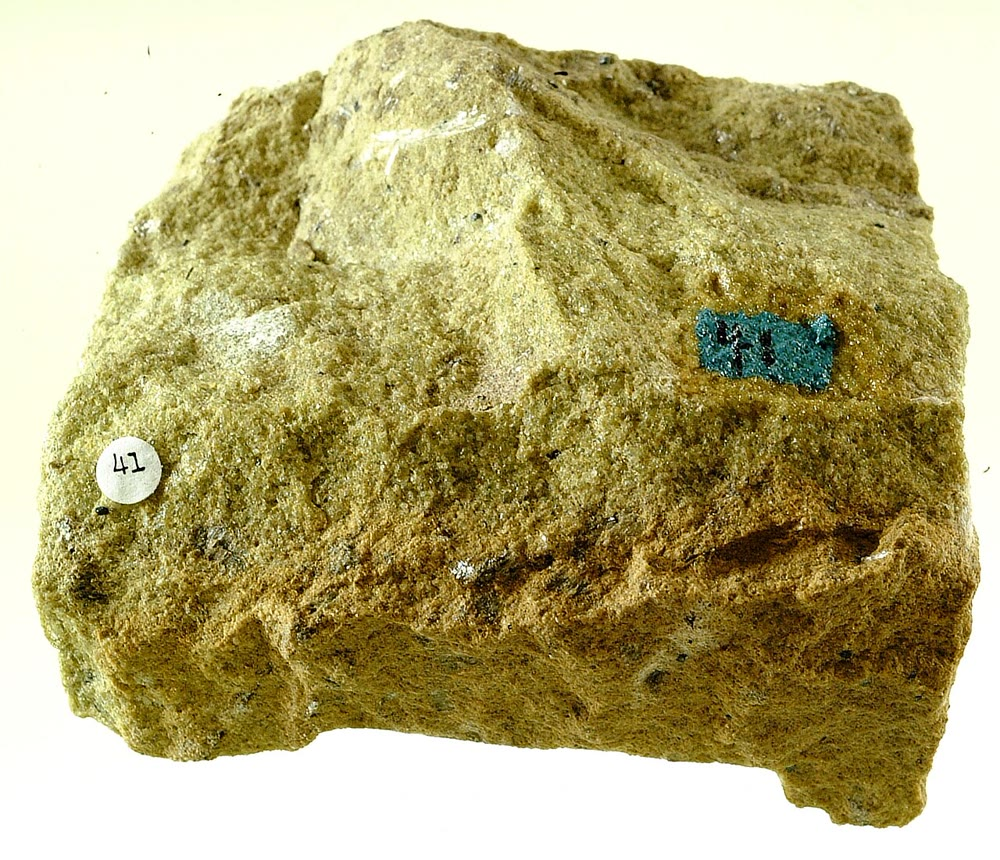
\includegraphics[width=\linewidth]{images/book4/b2-dunite.jpg}
\par\smallskip{\scriptsize A \omterm{def:b2:mantle-melting:peridotites}{dunite}, almost entirely olivine, with small black
grains of chromite; the sample is \qty{8.5}{cm} across (Mike Davis, CC0).}
\end{minipage}
\end{inthefield}
% ledger: casetta23:kimberlite, tulane:ocean-basins (Book 2), bgs:ultramafic

\section{Exercises}

\begin{exercise}[$\star$]\label{exo:b2:mantle-melting:1}
Name each rock from its proportions of olivine, orthopyroxene and clinopyroxene
(per cent): (a) 93, 5, 2; (b) 75, 25, 0; (c) 60, 27, 13; (d) 30, 45, 25. (e) Give
the name of the model upper mantle (57, 28, 13 and \qty{2}{\percent} spinel) after
renormalising its three silicates to \qty{100}{\percent}.
\end{exercise}
% ledger: bgs:ultramafic, liang21:dmm-mode

\begin{exercise}[$\star$]\label{exo:b2:mantle-melting:2}
On the diopside--anorthite diagram, a liquid of \qty{60}{\percent} anorthite
cools. (a) At what temperature does it begin to crystallise, and which mineral
forms? (b) At what temperature does the second mineral appear, and what is then
the composition of the liquid? (c) What is the composition of the first liquid when
a rock of \qty{80}{\percent} diopside and \qty{20}{\percent} anorthite is heated,
and at what temperature does it appear?
\end{exercise}
% ledger: bowen15:di-an

\begin{exercise}[$\star$]\label{exo:b2:mantle-melting:3}
(a) Compute the adiabatic gradient $\alpha T/(\rho c_p)$ in kelvins per gigapascal
for $T_p = \qty{1350}{\celsius}$, $\alpha = \qty{4.0e-5}{K^{-1}}$, $\rho =
\qty{3300}{kg/m^3}$, $c_p = \qty{1000}{J/(kg.K)}$. (b) How many kilometres of
mantle make a gigapascal ($g = \qty{9.81}{m/s^2}$)? Convert the gradient to kelvins
per kilometre and compare with a typical geothermal gradient near the surface,
about \qty{30}{K/km}.
\end{exercise}
% ledger: katz03:thermo, earle:settings (Book 2)

\begin{exercise}[$\star$]\label{exo:b2:mantle-melting:4}
(a) Compute the dry solidus of \omterm{def:b2:mantle-melting:peridotites}{peridotite} at 0, 1, 2 and \qty{3}{GPa}. (b) By how
many degrees does it rise per gigapascal near \qty{2}{GPa}? (c) Explain in one
sentence why a mantle at \qty{1400}{\celsius} at \qty{3}{GPa} is solid, and the
same mantle brought to \qty{2}{GPa} without exchanging heat is partly molten.
\end{exercise}
% ledger: katz03:solidus

\begin{exercise}[$\star\star$]\label{exo:b2:mantle-melting:5}
A liquid of \qty{70}{\percent} diopside and \qty{30}{\percent} anorthite cools.
(a) Estimate its liquidus temperature by interpolating between the liquidus at
\qty{20}{\percent} anorthite (\qty{1350}{\celsius}) and at \qty{40}{\percent}
(\qty{1277.5}{\celsius}). (b) Which mineral crystallises first? (c) What mass
fraction of the system has crystallised when the liquid reaches the eutectic?
(d) What are the proportions of diopside and anorthite in the final rock?
\end{exercise}
% ledger: bowen15:di-an

\begin{exercise}[$\star\star$]\label{exo:b2:mantle-melting:6}
(a) Compute the mass percentage of \ce{SiO2} in forsterite \ce{Mg2SiO4} and in
enstatite \ce{MgSiO3} ($M_{\ce{MgO}} = \qty{40.30}{g/mol}$, $M_{\ce{SiO2}} =
\qty{60.08}{g/mol}$). (b) Bowen and Andersen found the peritectic liquid to be
\qty{97.5}{\percent} \ce{MgSiO3} and \qty{2.5}{\percent} \ce{SiO2}: what is its
silica content? (c) Use the lever rule to compute the mass fraction of forsterite
formed when enstatite melts at the peritectic, and compare with their
\qty{5.5}{\percent}. (d) What does this imply for the silica content of a melt of
\omterm{def:b2:mantle-melting:peridotites}{peridotite} compared with that of its orthopyroxene?
\end{exercise}
% ledger: bowen14:mgo-sio2

\begin{exercise}[$\star\star$]\label{exo:b2:mantle-melting:7}
With the adiabat $T = T_p + 20P$ and the dry solidus of the text, compute the
pressure and the depth ($\qty{30.9}{km}$ per gigapascal) at which melting begins
for (a) $T_p = \qty{1300}{\celsius}$ and (b) $T_p = \qty{1450}{\celsius}$. (c) By
how many kilometres per \qty{10}{\celsius} does the onset deepen near
$T_p = \qty{1300}{\celsius}$? Use \cref{prop:b2:mantle-melting:onset}.
\end{exercise}
% ledger: katz03:solidus

\begin{exercise}[$\star\star$]\label{exo:b2:mantle-melting:8}
At \qty{2.0}{GPa}, take the \omterm{def:b2:mantle-melting:fraction}{melt fraction} to rise linearly from the dry solidus to
the \omterm{def:b2:mantle-melting:peridotites}{lherzolite} liquidus $T_{\mathrm l} = 1475.0 + 80.0P - 3.2P^2$. For $F = 0.10$:
(a) compute the temperature of the melting rock; (b) compute $(\partial
T/\partial P)_F$ and $(\partial T/\partial F)_P$; (c) compute the productivity with
$c_p = \qty{1000}{J/(kg.K)}$, $\alpha/\rho = \qty{1.21e-8}{m^3/(kg.K)}$ and
$\Delta S = \qty{300}{J/(kg.K)}$. (d) What would it be without latent heat?
\end{exercise}
% ledger: katz03:solidus, katz03:melting, katz03:thermo

\begin{exercise}[$\star\star$]\label{exo:b2:mantle-melting:9}
(a) By how much do 1, 5 and \qty{13}{\percent} of water dissolved in the melt lower
the solidus? (b) What is the water-saturated solidus at \qty{1}{GPa}? (c) A mantle
holds \qty{125}{ppm} of water by mass, and water's partition coefficient between
minerals and melt is 0.01. At the very first melting, the melt holds $X =
X_{\text{bulk}}/D$: compute it and the solidus lowering it causes.
\end{exercise}
% ledger: katz03:water

\begin{exercise}[$\star\star\star$]\label{exo:b2:mantle-melting:10}
(a) In \cref{prop:b2:mantle-melting:triangle}, check that the mantle entering the
base of the triangle each year equals the mantle leaving across its sides. Why
must the sides be at \ang{45} for a mantle that rises at $U$ and leaves at $U$?
(b) Show that, with constant productivity $\Pi$ per gigapascal, $h_c = \Pi\,\rho
g\,z_0^2/2$ (with $P_0 = \rho g z_0$), so that the crust grows as the square of the
depth of the onset. (c) A ridge spreads at a full rate of \qty{50}{mm/yr} and
makes \qty{7.1}{km} of crust: what volume of crust does each kilometre of ridge
make per year, and what volume of mantle does it melt if the mean \omterm{def:b2:mantle-melting:fraction}{melt fraction} is
\qty{12}{\percent}?
\end{exercise}

\begin{exercise}[$\star\star\star$]\label{exo:b2:mantle-melting:11}
In the ternary system of the schematic figure, the liquid $X$ has
\qty{60}{\percent} A, \qty{20}{\percent} B and \qty{20}{\percent} C; the
binary eutectic $e_{AB}$ is at A 40, B 60 (per cent), and the \omterm{def:b2:mantle-melting:ternary}{ternary eutectic} E at
A 25, B 30, C 45. (a) Write the composition of the liquid when a mass fraction $t$
of pure A has crystallised, and show that the ratio of B to C stays at 1. (b) The
cotectic from $e_{AB}$ to E is the line of points $e_{AB} + s(E - e_{AB})$: find
where the liquid meets it, and the fraction of A crystallised by then. (c) When
the liquid reaches E, what fraction of the system is still liquid? (C enters no
crystal before E.) (d) How much A and how much B have crystallised by then?
\end{exercise}

\begin{exercise}[$\star\star\star$]\label{exo:b2:mantle-melting:12}
The water content of a saturated melt is $X_{\mathrm{sat}} = 12P^{0.6} + P$
(per cent, $P$ in gigapascals). (a) Compute it at 1 and \qty{2}{GPa}, the solidus
lowering it gives, and the water-saturated solidus at both pressures. (b) Why does
the saturated solidus hardly change between 1 and \qty{2}{GPa} while the dry one
rises by more than \qty{100}{\celsius}? (c) In a mantle wedge at \qty{2}{GPa} and
\qty{1100}{\celsius}, how much water must the melt hold for the rock to melt?
\end{exercise}
% ledger: katz03:water, katz03:solidus

\section{Problem: Under the ridge}

\begin{problem}[{Weekend problem --- from the mantle adiabat to the thickness of
the oceanic crust, and back to the temperature of the mantle}]
\label{pb:b2:mantle-melting:1}
Mantle rises beneath a ridge along the adiabat and melts. Data: thermal
expansivity $\alpha = \qty{4.0e-5}{K^{-1}}$; density $\rho = \qty{3300}{kg/m^3}$;
specific heat $c_p = \qty{1000}{J/(kg.K)}$; entropy of melting $\Delta S =
\qty{300}{J/(kg.K)}$; $g = \qty{9.81}{m/s^2}$; dry solidus $T_{\mathrm s} =
1085.7 + 132.9P - 5.1P^2$ and \omterm{def:b2:mantle-melting:peridotites}{lherzolite} liquidus $T_{\mathrm l} = 1475.0 +
80.0P - 3.2P^2$ (\unit{\celsius}, $P$ in \unit{GPa}); mean productivity of the
fitted melting model, $\Pi = \qty{9}{\percent}$ per gigapascal; clinopyroxene
reaction coefficient near the surface 0.50; observed crust \qty[uncertainty-mode=separate]{7.1 \pm 0.8}{km}
at normal ridges and \qty{20}{km} over the core of the Iceland plume. Take mantle
and crust of the same density.

\noindent\textbf{Part I --- Where melting begins.}
\begin{enumerate}
\item Convert $T_p = \qty{1350}{\celsius}$ to kelvins.
\item Compute the adiabatic gradient $\alpha T_p/(\rho c_p)$ in kelvins per
gigapascal, and round it to the nearest ten.
\item How many kilometres of mantle make one gigapascal? Give the gradient in
kelvins per kilometre.
\item With the adiabat $T = 1350 + 20P$, write the quadratic for the onset pressure
$P_0$ and solve it.
\item Give the depth and the temperature at which melting begins.
\item Check that the solidus at $P_0$ gives the same temperature.
\end{enumerate}

\noindent\textbf{Part II --- How much melt.}
\begin{enumerate}[resume]
\item At \qty{1.5}{GPa}, compute the solidus, the \omterm{def:b2:mantle-melting:peridotites}{lherzolite} liquidus and their
difference.
\item With a \omterm{def:b2:mantle-melting:fraction}{melt fraction} rising linearly between them, give the temperature of
the rock at $F = 0.10$, in degrees Celsius and in kelvins.
\item Compute $(\partial T/\partial P)_F$ and $(\partial T/\partial F)_P$ there.
\item Compute the productivity of \cref{prop:b2:mantle-melting:productivity}, in
per cent per gigapascal.
\item The fitted model gives $\Pi = \qty{9}{\percent}$ per gigapascal on average.
Why is it lower? With $\Pi$, what is the \omterm{def:b2:mantle-melting:fraction}{melt fraction} $F_{\max}$ reached at the
surface?
\item The model mantle holds \qty{13}{\percent} clinopyroxene. At what \omterm{def:b2:mantle-melting:fraction}{melt
fraction} is it used up near the surface? Is the residue beneath the axis a
\omterm{def:b2:mantle-melting:peridotites}{lherzolite} or a \omterm{def:b2:mantle-melting:peridotites}{harzburgite}?
\end{enumerate}

\noindent\textbf{Part III --- The crust.}
\begin{enumerate}[resume]
\item Use \cref{prop:b2:mantle-melting:triangle} with $H = z_0$ to compute the
thickness of the crust.
\item What is the mean \omterm{def:b2:mantle-melting:fraction}{melt fraction} of the aggregated melt?
\item Compare with the observed thickness.
\item The full model of the figure gives \qty{9.0}{km}. Why is it thinner than
your estimate?
\item Show that $h_c = k P_0^2$ and compute $k$ in kilometres per square
gigapascal.
\end{enumerate}

\noindent\textbf{Part IV --- The temperature of the mantle.}
\begin{enumerate}[resume]
\item Compute the onset pressure $P_0$ that makes \qty{7.1}{km} of crust.
\item Give the corresponding depth of the onset.
\item With the adiabat $T = T_p + 20P$, compute the potential temperature that
puts the onset at that pressure.
\item Redo the calculation for 6.3 and \qty{7.9}{km}: what range of $T_p$ does the
scatter of the crust allow?
\item The crust is \qty{20}{km} thick over the core of the Iceland plume. Compute
the potential temperature there, and its excess over that of question~20.
\item Lavas of ocean islands suggest plumes 200 to \qty{300}{\celsius} hotter than
the ambient mantle. Suggest why the crust gives a smaller excess.
\item By how many per cent does the crust thicken for a mantle \qty{10}{\celsius}
hotter, near the normal ridge?
\item Very slow ridges make thinner crust. Explain why with the triangle.
\item State the potential temperature of the mantle beneath a normal ridge that
the thickness of the crust gives, the key number of this problem, and compare
it with the \qty{1350}{\celsius} from mineral physics and the range 1280 to
\qty{1400}{\celsius} from lavas.
\end{enumerate}
\end{problem}
% ledger: katz03:solidus, katz03:melting, katz03:thermo, white:crust (Book 3), herzberg:tp (Book 3), katsura:adiabat (Book 3)
